\section{Análisis de Resultados}

En esta sección se dará respuesta y explicación de los resultados de la sección pasada. Es importante decir que se harán referencia a las Figuras mostradas en la sección anterior, por lo que se hará necesario volver a revisarlas en cierto punto. 

\subsection{Capa física y de enlace : Análisis de la red}

\noindent En la sección pasada se vio como se utilizaba la
herramienta \verb|iperf3| y \verb|nmap| para escanear la red en busca de sus dispositivos. De este escaneo, se obtuvo la tabla/cuadro \ref{if} con los 9 dispositivos conectados a la red. Pero de esto surge la siguiente duda ¿Cuantos dispositivos pueden estar conectados a la red ?, Una respuesta rápida seria tantos como la cantidad de ips pueda dar el router. \cite{maxMAC}. Entonces en el caso particular la cantidad maxima de dispositivos que puede aceptar el router son 253 (del 1 al 255, menos un que es utilizado por el propio router). Sin embargo, no es recomendable tener tantos dispositivos conectados debido al tráfico que generaría, ralentizando la velocidad de transferencia.
\newline

\noindent Ahora si se fija en la figura \ref{diag:red} que muestra el diagrama de red, se puede ver que un detalle de los dispositivos conectados tanto por Wifi y por Ethernet, cabe destacar que como el router trabaja con dual band en la señal wifi(2.4GHz y 5GHz), algunos dispositivos terminan conectándose a la señal por un protocolo distinto, por ejemplo, los dispositivos que se conectan al 5G utilizan 802.11a mientras que los que se conectan al 2.4G utilizan 802.11b/g/n/ac. También en este diagrama tiene un foco en la distribución interna de los dispositivos, ahora si se quiere saber más sobre lo que ocurre fuera del hogar, se puede investigar desde la página del proveedor de internet. En este caso sería \textbf{Mundo pacifico}.


\begin{figure}[!h]
	\centering
	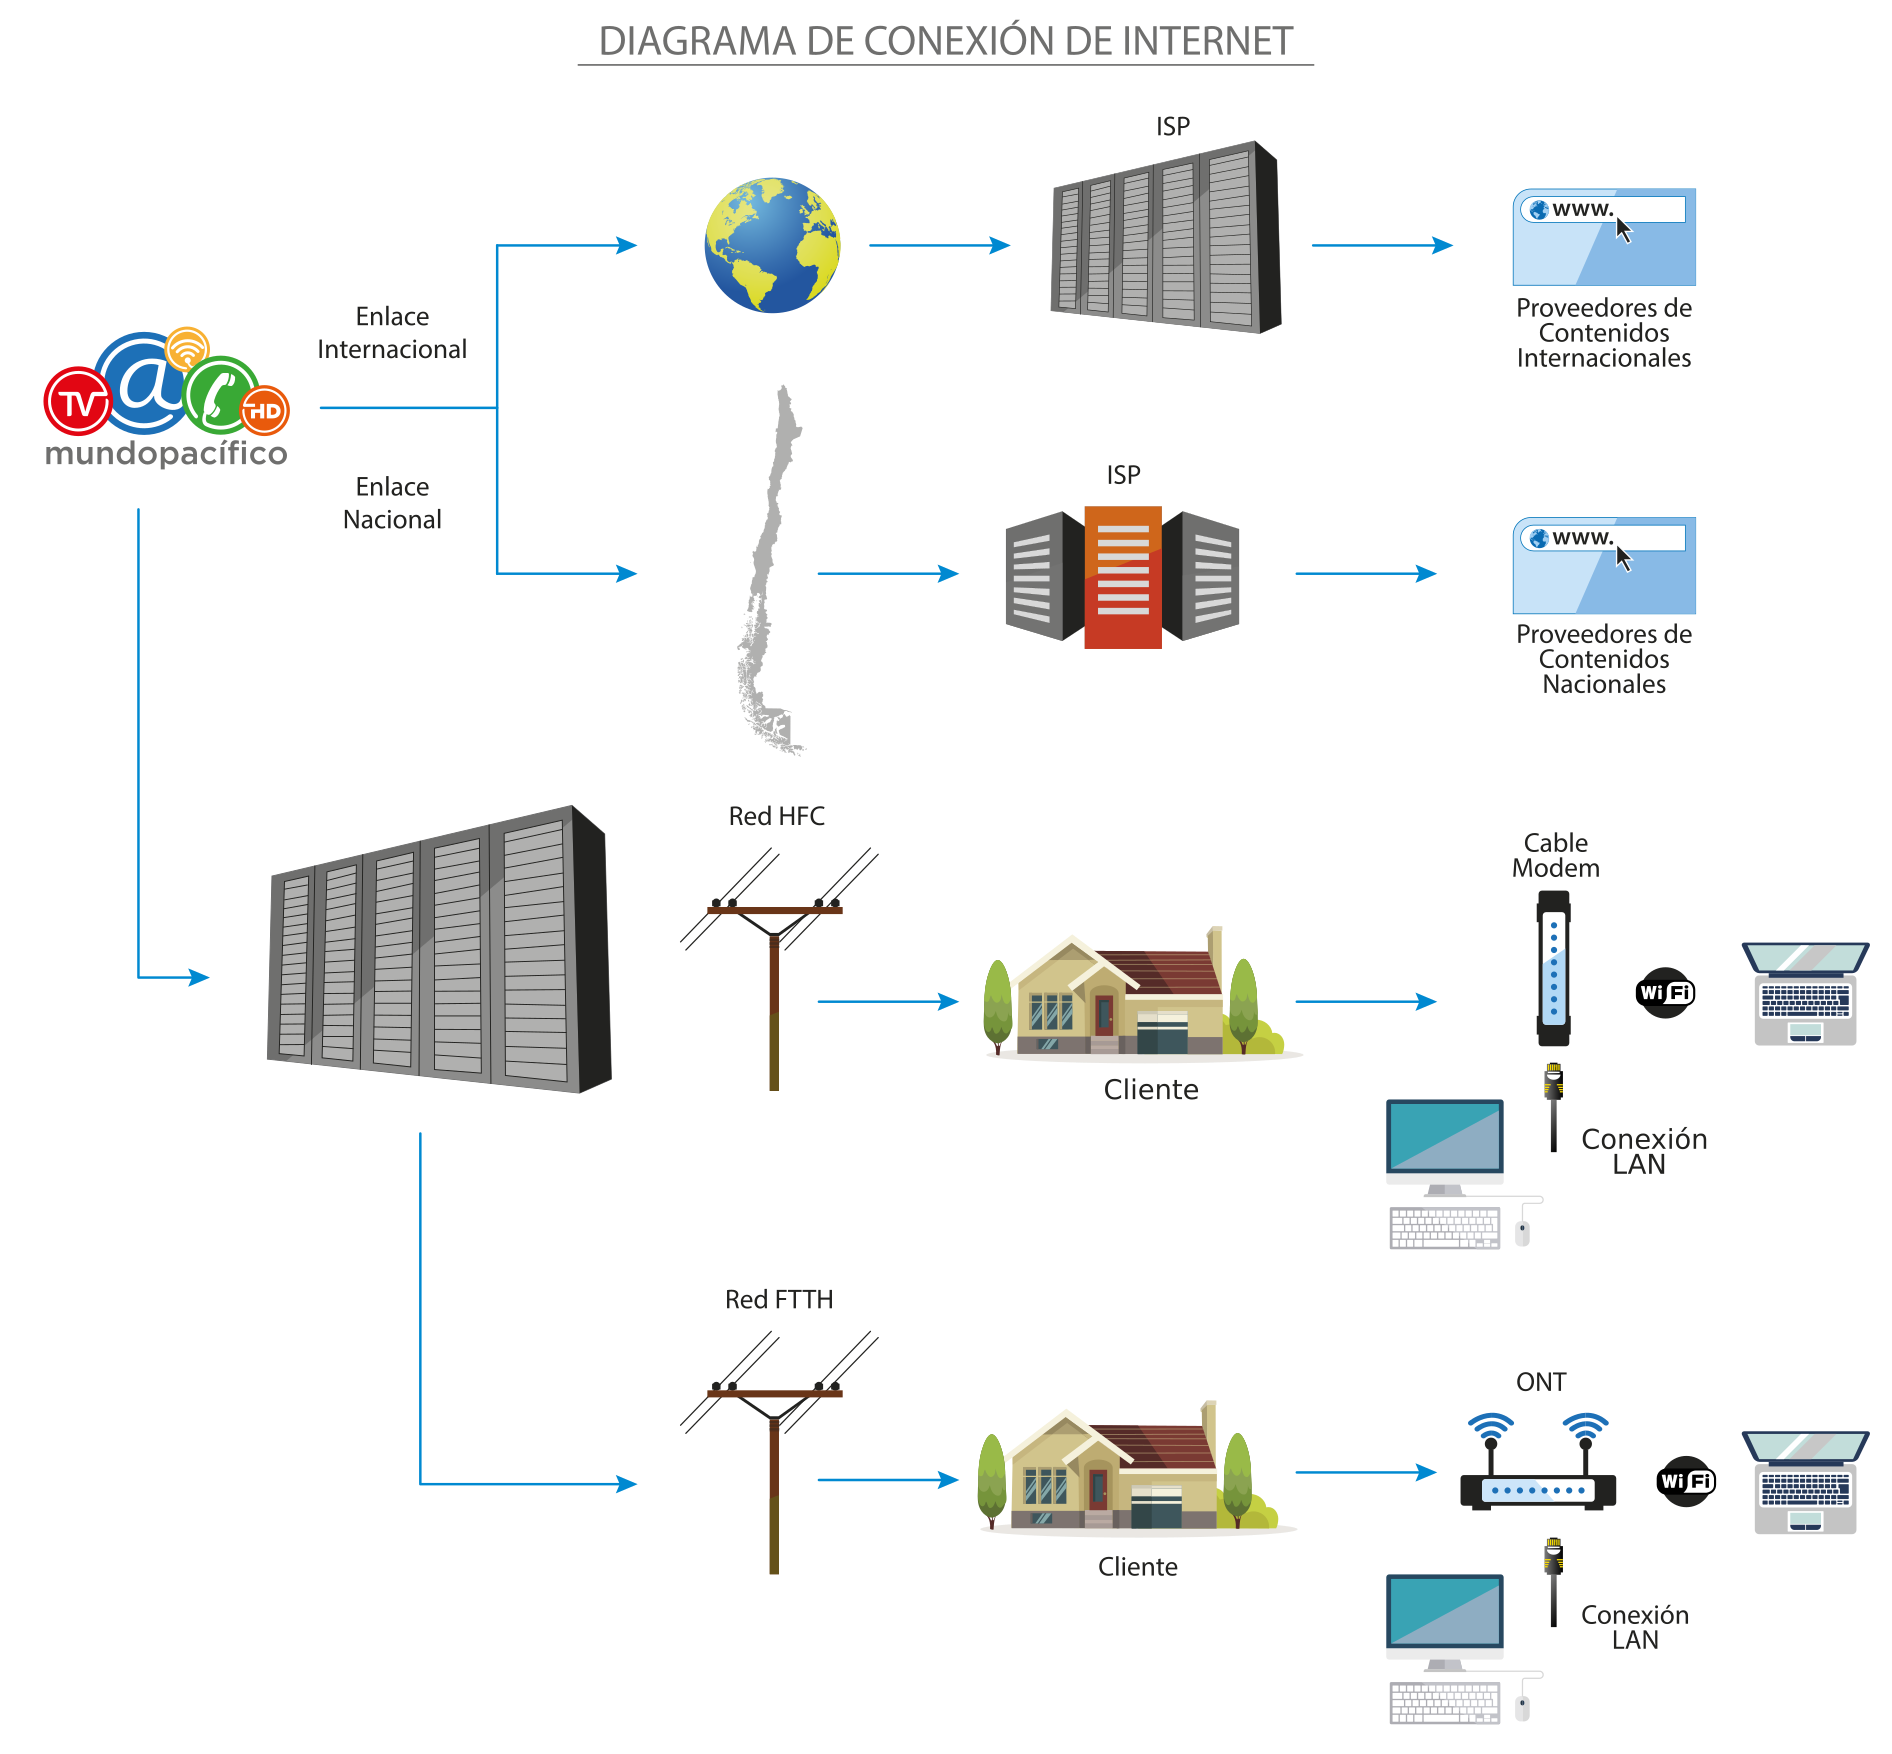
\includegraphics[scale=0.9]{images/diagrama-conexxion-net.png}
	\caption{Diagrama de conexión a internet fuera del hogar obtenido de Mundo Pacifico \cite{Mundo} }
	\label{diag:iperf3}
\end{figure}

\noindent Como se vio en la sección anterior, se ha realizado un test de velocidad entre los dispositivos \textbf{PC-Escritorio} (\verb|192.168.18.5|) que actúa como server y \textbf{NENVY13} (\verb|192.168.18.8|), el cual es donde se envían los paquetes. El resultado de dicho test se encuentra en el gráfico de la figura \ref{diag:iperf3} el cual si se analiza se puede ver que a primera vista no existe alguna relación con la tasa de pérdidas y el ancho de banda, además es importante mencionar el dispositivo NENVY13 se encontraba conectado al 5G del router, alcanzando una velocidad máxima de 425 Mbits/s entonces en la prueba de ancho de banda de 500 y 1000 no hubo diferencia de velocidad. Luego de esto surge la pregunta ¿Existirá alguna diferencia de la tasa de perdidas con el tipo de protocolo usando en la conexión? Para esto se ha repetido la experiencia, pero se ha conectado el dispositivo NENVY13 a la red 2.4G. Como resultado ha dado lo siguiente: 

\newpage

\begin{figure}[!h]
	\centering
	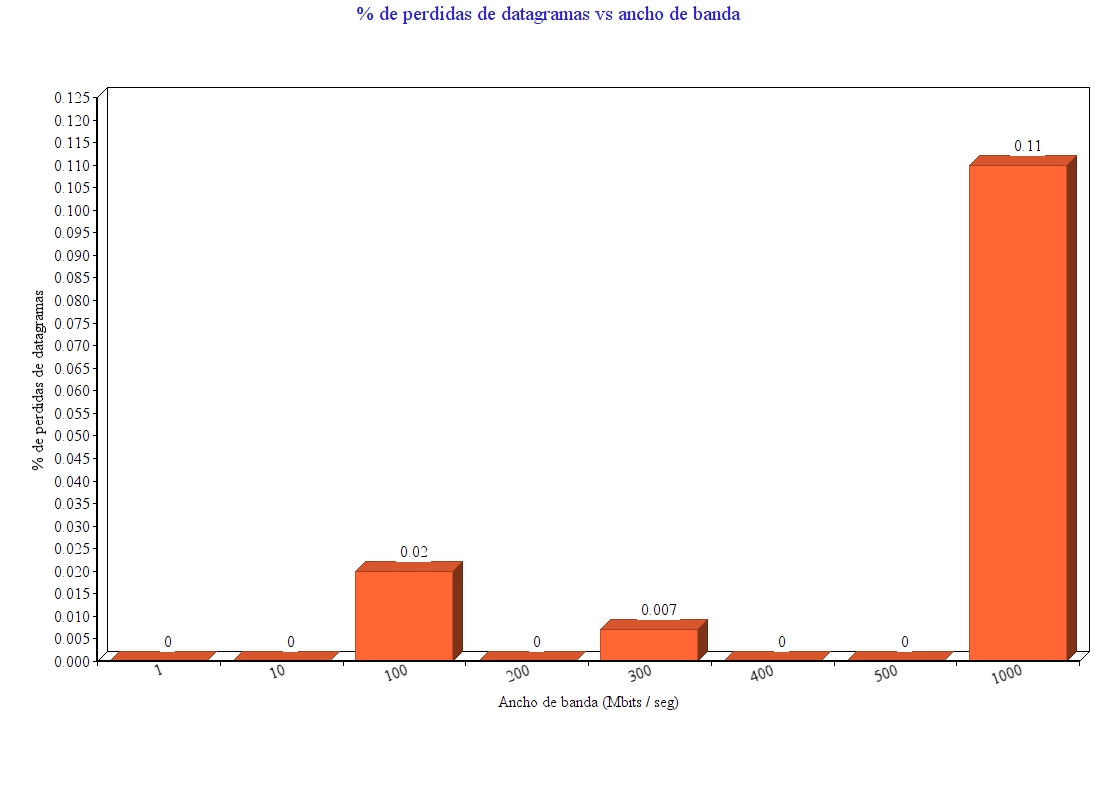
\includegraphics[scale=0.5]{images/barplots.png}
	\caption{Gráfico del \% de datagramas perdidos v/s Ancho de banda en 2.4G}
	\label{diag:iperf3}
\end{figure}

\noindent Como se puede ver la cantidad de Datagramas perdidos ha descendido de forma considerable, teniendo solo un máximo de 0.11\%, cabe destacar que la velocidad máxima alcanzada fue de 110 Mbits/s. Lo anterior puede significar que el 5G es mucho más inestable en cuanto a la transmisión que el 2.4G, sin embargo, su velocidad es mucha mayor a la del 2.4G.

\newline

\noindent Respecto a los datagramas, estos se pierden debido a las colisiones que existen dentro de la red, por ejemplo, si estuvieran solo estos 2 equipos en la red, habría una menor probabilidad de tener perdidas de datagramas. 

\subsection{Protocolo ARP}

Como se vio en el capítulo anterior, al momento de hacer de estar revisando las tablas ARP y vaciarlas, se puede ver en la figura \ref{fig:arp1} que la tabla si contiene algunas ips ¿Esto por qué se da?, primeramente si se ven las ips en la tabla se puede diferenciar la primera (\verb|192.168.18.1|), si se recuerda, esta ip corresponde a la ip del router por lo que es necesario que exista en la tabla ARP ya que el router siempre se está comunicando con el dispositivo.  Ahora la segunda ip (\verb|192.168.18.6|) corresponde a la ip del dispositivo de Google home mini. A primera vista, no se puede establecer una explicación de por qué se encuentra en la tabla ARP. Investigando un poco, este dispositivo escanea constantemente la red en busca de otros dispositivos compatibles con la integración de Google, entonces este dispositivo posee la información de cada equipo conectado a la red en su tabla ARP. 
\newline

\noindent Después de esta explicación, al momento de hacer ping a un dispositivo, el protocolo hace necesario guardar en la tabla ARP la información del dispositivo que está haciendo ping. Entonces cualquier dispositivo que haga ping a otro dentro de la red, este último sabrá quién le está mandando información ya que lo tendrá agregado a su propia tabla, lo cual explica la figura \ref{fig:arp2}. 


\noindent Ahora bien, una cosa es saber que ocurre dentro de cada dispositivo pero ¿Que ocurre en la red cuando se envía un ping a un dispositivo? Para responder esta pregunta, es necesario utilizar Wireshark, y colocar el siguiente filtro \verb|ip.dst==192.168.18.8|, lo cual fija la ip de destino del dispositivo NENVY13. 


\begin{figure}[!h]
	\centering
	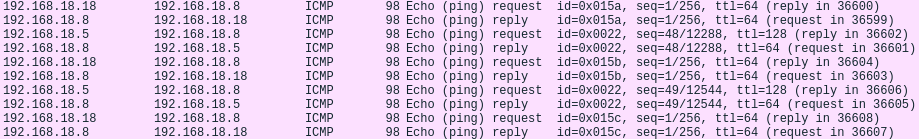
\includegraphics[scale=0.5]{images/wire3.png}
	\caption{Imagen de lo que ocurre en Wireshark mientras se realizan los ping al equipo NENVY13}
	\label{diag:iperf3}
\end{figure}

\noindent Como se puede ver para la comunicación se utiliza el protocolo ICMP, el cual es sirve para mandar mensajes entre dos dispositivos con información sobre el estado de la red y devolver mensajes sobre problemas con datagramas al remitente del paquete \cite{icmp}. En este caso lo que se envía es una información de control y por el comando: \verb|echo (ping)|. 

\noindent Si se ve en la info , se puede notar que cada paquete de ping es acompañado de un \textit{Request} o \textit{Reply} dependiendo en qué dirección vaya. Si el destino es \verb|echo (ping)| será una \textit{Request} caso contrario, si el inicio es \verb|echo (ping)| será una \textit{Reply} .
\newline

\noindent Se se analiza el tráfico general de la red se puede ver que este es normal y se puede notar que la mayor cantidad de paquetes son enviados desde el dispositivo \textbf{Google home mini} ya sea a los dispositivos conectados como a los servidores de Google, en específico se hacen a la ip \verb|172.217.192.97| la cual con cualquier \textit{Whois} en internet se puede saber a quién pertenece.
